%% (Master) Thesis template
% Template version used: v1.4
%
% Largely adapted from Adrian Nievergelt's template for the ADPS
% (lecture notes) project.


%% We use the memoir class because it offers a many easy to use features.
\documentclass[11pt,a4paper,titlepage,oldfontcommands]{memoir}


%% Packages

%% ========

%% LaTeX Font encoding -- DO NOT CHANGE
\usepackage[OT1]{fontenc}

%% Babel provides support for languages.  'english' uses British
%% English hyphenation and text snippets like "Figure" and
%% "Theorem". Use the option 'ngerman' if your document is in German.
%% Use 'american' for American English.  Note that if you change this,
%% the next LaTeX run may show spurious errors.  Simply run it again.
%% If they persist, remove the .aux file and try again.
\usepackage[english]{babel}

%% Input encoding 'utf8'. In some cases you might need 'utf8x' for
%% extra symbols. Not all editors, especially on Windows, are UTF-8
%% capable, so you may want to use 'latin1' instead.
\usepackage[utf8]{inputenc}

%% This changes default fonts for both text and math mode to use Herman Zapfs
%% excellent Palatino font.  Do not change this.
\usepackage[sc]{mathpazo}

%% The AMS-LaTeX extensions for mathematical typesetting.  Do not
%% remove.
\usepackage{amsmath,amssymb,amsfonts,mathrsfs}

%% NTheorem is a reimplementation of the AMS Theorem package. This
%% will allow us to typeset theorems like examples, proofs and
%% similar.  Do not remove.
%% NOTE: Must be loaded AFTER amsmath, or the \qed placement will
%% break
\usepackage[amsmath,thmmarks]{ntheorem}

%% LaTeX' own graphics handling
\usepackage{graphicx}

%% We unfortunately need this for the Rules chapter.  Remove it
%% afterwards; or at least NEVER use its underlining features.
\usepackage{soul}

%% This allows you to add .pdf files. It is used to add the
%% declaration of originality.
\usepackage{pdfpages}

%% Some more packages that you may want to use.  Have a look at the
%% file, and consult the package docs for each.
%% See the TeXed file for more explanations

%% [OPT] Multi-rowed cells in tabulars
%\usepackage{multirow}

%% [REC] Intelligent cross reference package. This allows for nice
%% combined references that include the reference and a hint to where
%% to look for it.
\usepackage{varioref}

%% [OPT] Easily changeable quotes with \enquote{Text}
%\usepackage[german=swiss]{csquotes}

%% [REC] Format dates and time depending on locale
\usepackage{datetime}

%% [OPT] Provides a \cancel{} command to stroke through mathematics.
%\usepackage{cancel}

%% [NEED] This allows for additional typesetting tools in mathmode.
%% See its excellent documentation.
\usepackage{mathtools}

%% [ADV] Conditional commands
%\usepackage{ifthen}

%% [OPT] Manual large braces or other delimiters.
%\usepackage{bigdelim, bigstrut}

%% [REC] Alternate vector arrows. Use the command \vv{} to get scaled
%% vector arrows.
\usepackage[h]{esvect}

%% [NEED] Some extensions to tabulars and array environments.
\usepackage{array}

%% [OPT] Postscript support via pstricks graphics package. Very
%% diverse applications.
%\usepackage{pstricks,pst-all}

%% [?] This seems to allow us to define some additional counters.
%\usepackage{etex}

%% [ADV] XY-Pic to typeset some matrix-style graphics
%\usepackage[all]{xy}

%% [OPT] This is needed to generate an index at the end of the
%% document.
%\usepackage{makeidx}

%% [OPT] Fancy package for source code listings.  The template text
%% needs it for some LaTeX snippets; remove/adapt the \lstset when you
%% remove the template content.
\usepackage{listings}
\lstset{language=TeX,basicstyle={\normalfont\ttfamily}}

%% [REC] Fancy character protrusion.  Must be loaded after all fonts.
\usepackage[activate]{pdfcprot}

%% [REC] Nicer tables.  Read the excellent documentation.
\usepackage{booktabs}


%% Our layout configuration.  DO NOT CHANGE.
%% Memoir layout setup

%% NOTE: You are strongly advised not to change any of them unless you
%% know what you are doing.  These settings strongly interact in the
%% final look of the document.

% Dependencies
\usepackage{ETHlogo}

% Turn extra space before chapter headings off.
\setlength{\beforechapskip}{0pt}

\nonzeroparskip
\parindent=0pt
\defaultlists

% Chapter style redefinition
\makeatletter

\if@twoside
  \pagestyle{Ruled}
  \copypagestyle{chapter}{Ruled}
\else
  \pagestyle{ruled}
  \copypagestyle{chapter}{ruled}
\fi
\makeoddhead{chapter}{}{}{}
\makeevenhead{chapter}{}{}{}
\makeheadrule{chapter}{\textwidth}{0pt}
\copypagestyle{abstract}{empty}

\makechapterstyle{bianchimod}{%
  \chapterstyle{default}
  \renewcommand*{\chapnamefont}{\normalfont\Large\sffamily}
  \renewcommand*{\chapnumfont}{\normalfont\Large\sffamily}
  \renewcommand*{\printchaptername}{%
    \chapnamefont\centering\@chapapp}
  \renewcommand*{\printchapternum}{\chapnumfont {\thechapter}}
  \renewcommand*{\chaptitlefont}{\normalfont\huge\sffamily}
  \renewcommand*{\printchaptertitle}[1]{%
    \hrule\vskip\onelineskip \centering \chaptitlefont\textbf{\vphantom{gyM}##1}\par}
  \renewcommand*{\afterchaptertitle}{\vskip\onelineskip \hrule\vskip
    \afterchapskip}
  \renewcommand*{\printchapternonum}{%
    \vphantom{\chapnumfont {9}}\afterchapternum}}

% Use the newly defined style
\chapterstyle{bianchimod}

\setsecheadstyle{\Large\bfseries\sffamily}
\setsubsecheadstyle{\large\bfseries\sffamily}
\setsubsubsecheadstyle{\bfseries\sffamily}
\setparaheadstyle{\normalsize\bfseries\sffamily}
\setsubparaheadstyle{\normalsize\itshape\sffamily}
\setsubparaindent{0pt}

% Set captions to a more separated style for clearness
\captionnamefont{\sffamily\bfseries\footnotesize}
\captiontitlefont{\sffamily\footnotesize}
\setlength{\intextsep}{16pt}
\setlength{\belowcaptionskip}{1pt}

% Set section and TOC numbering depth to subsection
\setsecnumdepth{subsection}
\settocdepth{subsection}

%% Titlepage adjustments
\pretitle{\vspace{0pt plus 0.7fill}\begin{center}\HUGE\sffamily\bfseries}
\posttitle{\end{center}\par}
\preauthor{\par\begin{center}\let\and\\\Large\sffamily}
\postauthor{\end{center}}
\predate{\par\begin{center}\Large\sffamily}
\postdate{\end{center}}

\def\@advisors{}
\newcommand{\advisors}[1]{\def\@advisors{#1}}
\def\@department{}
\newcommand{\department}[1]{\def\@department{#1}}
\def\@thesistype{}
\newcommand{\thesistype}[1]{\def\@thesistype{#1}}

\renewcommand{\maketitlehooka}{\noindent\ETHlogo[2in]}

\renewcommand{\maketitlehookb}{\vspace{1in}%
  \par\begin{center}\Large\sffamily\@thesistype\end{center}}

\renewcommand{\maketitlehookd}{%
  \vfill\par
  \begin{flushright}
    \sffamily
    \@advisors\par
    \@department, ETH Z\"urich
  \end{flushright}
}

\checkandfixthelayout

\setlength{\droptitle}{-48pt}

\makeatother

% This defines how theorems should look. Best leave as is.
\theoremstyle{plain}
\setlength\theorempostskipamount{0pt}

%%% Local Variables:
%%% mode: latex
%%% TeX-master: "thesis"
%%% End:


%% Theorem environments.  You will have to adapt this for a German
%% thesis.
%% Theorem-like environments

%% This can be changed according to language. You can comment out the ones you
%% don't need.

\numberwithin{equation}{chapter}

%% German theorems
%\newtheorem{satz}{Satz}[chapter]
%\newtheorem{beispiel}[satz]{Beispiel}
%\newtheorem{bemerkung}[satz]{Bemerkung}
%\newtheorem{korrolar}[satz]{Korrolar}
%\newtheorem{definition}[satz]{Definition}
%\newtheorem{lemma}[satz]{Lemma}
%\newtheorem{proposition}[satz]{Proposition}

%% English variants
\newtheorem{theorem}{Theorem}[chapter]
\newtheorem{example}[theorem]{Example}
\newtheorem{remark}[theorem]{Remark}
\newtheorem{corollary}[theorem]{Corollary}
\newtheorem{definition}[theorem]{Definition}
\newtheorem{lemma}[theorem]{Lemma}
\newtheorem{proposition}[theorem]{Proposition}

%% Proof environment with a small square as a "qed" symbol
\theoremstyle{nonumberplain}
\theorembodyfont{\normalfont}
\theoremsymbol{\ensuremath{\square}}
\newtheorem{proof}{Proof}
%\newtheorem{beweis}{Beweis}


%% Helpful macros.
%% Custom commands
%% ===============

%% Special characters for number sets, e.g. real or complex numbers.
\newcommand{\C}{\mathbb{C}}
\newcommand{\K}{\mathbb{K}}
\newcommand{\N}{\mathbb{N}}
\newcommand{\Q}{\mathbb{Q}}
\newcommand{\R}{\mathbb{R}}
\newcommand{\Z}{\mathbb{Z}}
\newcommand{\X}{\mathbb{X}}

%% Fixed/scaling delimiter examples (see mathtools documentation)
\DeclarePairedDelimiter\abs{\lvert}{\rvert}
\DeclarePairedDelimiter\norm{\lVert}{\rVert}

%% Use the alternative epsilon per default and define the old one as \oldepsilon
\let\oldepsilon\epsilon
\renewcommand{\epsilon}{\ensuremath\varepsilon}

%% Also set the alternate phi as default.
\let\oldphi\phi
\renewcommand{\phi}{\ensuremath{\varphi}}




%% Make document internal hyperlinks wherever possible. (TOC, references)
%% This MUST be loaded after varioref, which is loaded in 'extrapackages'
%% above.  We just load it last to be safe.
\usepackage[linkcolor=black,colorlinks=true,citecolor=black,filecolor=black]{hyperref}


%% Document information
%% ====================

\title{Title of Thesis}
\author{Ramapriya Sridharan}
\thesistype{Master Thesis}
\advisors{Advisors: Prof.\ Dr.\ Dirk Helbing, Dr.\ Pournaras Evangelos}
\department{Department of Computational Social Sciences }
\date{September 3, 2016}

\begin{document}

\frontmatter

%% Title page is autogenerated from document information above.  DO
%% NOT CHANGE.
\begin{titlingpage}
  \calccentering{\unitlength}
  \begin{adjustwidth*}{\unitlength-24pt}{-\unitlength-24pt}
    \maketitle
  \end{adjustwidth*}
\end{titlingpage}

%% The abstract of your thesis.  Edit the file as needed.
%%ngo\begin{abstract}
Today, there are unrestricted opportunities for people to generate and share their data in real time with the advent of Internet of Things, ubiquitous and pervasive computing \cite{pournarasethical}. Due to the unstructured nature, variability and rate of growth of this data when it is recorded, analysed and processed efficiently, it can lead to the understanding of one's business or competitors that leads to better products and services. Jinyan Zang et al \cite{zang2015knows} and Ashwini Rao et al \cite{rao2015they} talk about the non transparent ways of today's data collection systems where people are uninformed about the data collection process.

This Thesis builds upon the paper by Pournaras et al \cite{pournaras2016self} where data sharing is modelled as a supply-demand system. The concept of a computational market is introduced where data aggregators who analyse data can incentivize people to share their data with a certain accuracy and this is performed using summarization functions that regulate the amount of information in the data shared. There is lack of information on how people make decisions in the sharing of mobile sensor data. This information is needed in order to design a platform for a computational market that rewards users fairly and increases the awareness of people about their privacy.

In this Thesis, a social experiment and an Android application are designed to examine the relationship between mobile sensor data sharing and how incentives affect this. Users are requested for their data using data requests that are governed by three aspects: (a) sensor type, (b) the stakeholder to whom sensor data is shared, (c) the context or the application type for which data is shared. To do this, a computational model is introduced that assigns rewards to the possible data requests based on the user profiles formed by questioning users on the three aspects of data sharing. Data sharing decisions during the experiment are then tracked with and without incentives and the user data is recorded anonymously. The anonymous data recorded is then analysed and the findings can help in the making of platforms with fairer and more transparent data collection systems that make people more privacy aware.
\end{abstract}


%% TOC with the proper setup, do not change.
\cleartorecto
\tableofcontents
\mainmatter

%% Your real content!
%%\chapter{Introduction}

%In today's world, almost everybody owns a smartphone. Information collected from a large number of interconnected smartphones equipped with
%multiple number of sensors each can aid to accumulate large volumes of data which is heterogeneous and autonomous in nature. This large amounts of data in any form is called Big Data\footnote{Date:23-08-2016 \url{https://en.wikipedia.org/wiki/Big\_data}} and it
%is the stepping stone to large scale data analytics and Deep learning to understand the complexities in our society. 
%
%Currently, a lot of the data collected in mobile applications\footnote{Date:23-08-2016 \url{http://www.theregister.co.uk/2014/02/21/appthority\_app_privacy\_study}} and on the web\footnote{Date:23-08-2016 \url{http://www.techlicious.com/blog/whos-gathering-your-personal-information}}
%is done in a manner where users are unaware of the collection of their data. This process not only lacks transparency but also does not give users
%control over their data. Users should be able to make informed decisions about what data to share or not. Additionally, since no privacy algorithms 
%are implemented on the data collected, user privacies are at risk. Paul Ohm in his paper \cite{ohm2010broken} explains that it can be shown that anonymized data can be de-anonymized surprisingly easily. In this dissertation, focus is not given on the attacks such as hacking and any other methods but concentrated on the threats to the information in the data collected.
%
%The aim is to setup a fair way to collect data by setting up a platform over a participatory sensing network where users can trade their data for some incentives to stakeholders who approach them.
%Incentives can be money, vouchers or anything else. Stakeholders inform users about the date, duration for which data is collected, who will use the data and what will it be used for. Additionally, users have the possibility to share data with some added levels of privacy. 
%To achieve this goal, it is first essential to understand the relationship between incentives and mobile sensor data sharing. In this dissertation, a survey and social experiment is designed where a platform is created and users can trade and view their data in a transparent manner. Data from user inputs and decisions is collected and later analysed to throw light on user decision of their sensor data.


Big Data systems today often collect data in ways that are unfair, non transparent and privacy intrusive to people. Most of the times, people are unaware that data collection is taking place. For this reason, new ways of acquiring data need to be designed. People should have control over their data and be given all the necessary information before data collection such as: (i) Information about the data sharing process, (ii) Who will see the data, (iii) What data is collected, (iv) Time and duration of data collection, (v) What purpose is the data collected for. Addtionally to the above mentioned points, users should be given the choice to control the privacy or accuracy of the data they share. In additon to security threats to data, there are also threats to people's privacies due to the information content in the data shared. 

This Thesis builds upon the earlier work on self-regulatory information sharing in participatory social sensing by Pournaras et al \cite{pournaras2016self}. In this concept introduced, citizens who are suppliers are the ones sharing their data and they have the choice to choose how much of their data to share. On the other side, the data aggregators are the consumers who use the sensor data shared by citizens for some data analytics task. Data aggregators require data to be of some accuracy for their task and incentivize users accordingly to motivate them to share data with a certain level of accuracy. For example, if data aggregators would like data with a higher accuracy, they can incentivize citizens with higher incentive for sharing their data. Similarly, if the analysis task does not require data with high accuracy, lower incentives can be awarded to citizens for sharing data. Information content or accuracy of data can be regulated using summarization functions concerning algorithms from simple arithmetic functions to clustering algorithms. A high summarization level filters out most of the information in the data, hence preserving the privacy of the citizen. This can cause higher errors for the data aggregator. Similarly, a lower summarization level shows more information and causes less errors for the data aggregator.

To design a computational market platform where users can share data in a more transparent and fair manner, there is a lack of information on the choices users make in sharing their data. Additionally, there is a need to know the perception of citizens on the privacy of their mobile sensor data and this data will help understand the supply-demand system for data sharing. The findings from the above can help to create a fairer system for data collection. In order to cover this lack of information, a social experiment is designed where citizens are approached with data requests governed by the three following aspects:

\begin{itemize}
\item The sensor type
\item The stakeholder or entity requesting for citizen's sensor data
\item The context or purpose of sensor data collection
\end{itemize} 

The social experiment is carried out with an Android application and has an inbuilt computational model which assigns rewards to each data requests based on a citizen profile formed. This citizen profile is formed by asking citizens some questions regarding the three aspects mentioned above. Citizen decisions are recorded anonymously for later analysis. A pre survey is launched before the social experiment is carried out to understand the perception of users on the three aspects studied. An exit survey is also launched after the social experiment is finished to obtain feedback from citizens participating. 





%%\chapter{Writing scientific texts in English}

This chapter was originally a separate document written by Reto
Spöhel.  It is reprinted here so that the template can serve as a
quick guide to thesis writing, and to provide some more example
material to give you a feeling for good typesetting.

% We're going to need an extra theorem-like environment for this
% chapter
\theoremstyle{plain}
\theoremsymbol{}
\newtheorem{Rule}[theorem]{Rule}

\section{Basic writing rules}

The following rules need little further explanation; they are best
understood by looking at the example in the booklet by Knuth et al.,
§2--§3.

\begin{Rule}
  Write texts, not chains of formulas.
\end{Rule}

More specifically, write full sentences that are logically
interconnected by phrases like `Therefore', `However', `On the other
hand', etc.\ where appropriate.

\begin{Rule}
  Displayed formulas should be embedded in your text and punctuated
  with it.
\end{Rule}

In other words, your writing should not be divided into `text parts'
and `formula parts'; instead the formulas should be tied together by
your prose such that there is a natural flow to your writing.

\section{Being nice to the reader}

Try to write your text in such a way that a reader enjoys reading
it. That's of course a lofty goal, but nevertheless one you should
aspire to!

\begin{Rule}
  Be nice to the reader.
\end{Rule}

Give some intuition or easy example for definitions and theorems which
might be hard to digest. Remind the reader of notations you introduced
many pages ago -- chances are he has forgotten them. Illustrate your
writing with diagrams and pictures where this helps the reader. Etc.

\begin{Rule}
  Organize your writing.
\end{Rule}

Think carefully about how you subdivide your thesis into chapters,
sections, and possibly subsections.  Give overviews at the beginning
of your thesis and of each chapter, so the reader knows what to
expect. In proofs, outline the main ideas before going into technical
details. Give the reader the opportunity to `catch up with you' by
summing up your findings periodically.

\emph{Useful phrases:} `So far we have shown that \ldots', `It remains
to show that \ldots', `Recall that we want to prove inequality (7), as
this will allow us to deduce that \ldots', `Thus we can conclude that
\ldots. Next, we would like to find out whether \ldots', etc.

\begin{Rule}
  Don't say the same thing twice without telling the reader that you
  are saying it twice.
\end{Rule}

Repetition of key ideas is important and helpful. However, if you
present the same idea, definition or observation twice (in the same or
different words) without telling the reader, he will be looking for
something new where there is nothing new.

\emph{Useful phrases:} `Recall that [we have seen in Chapter 5 that]
\ldots', `As argued before / in the proof of Lemma 3, \ldots', `As
mentioned in the introduction, \ldots', `In other words, \ldots', etc.

\begin{Rule}
  Don't make statements that you will justify later without telling
  the reader that you will justify them later.
\end{Rule}

This rule also applies when the justification is coming right in the
next sentence!  The reasoning should be clear: if you violate it, the
reader will lose valuable time trying to figure out on his own what
you were going to explain to him anyway.

\emph{Useful phrases:} `Next we argue that \ldots', `As we shall see,
\ldots', `We will see in the next section that \ldots, etc.


\section{A few important grammar rules}

\begin{Rule}
  \label{rule:no-comma-before-that}
  There is (almost) \emph{never} a comma before `that'.
\end{Rule}

It's really that simple. Examples:
\begin{quote}
  We assume that \ldots\\
  \emph{Wir nehmen an, dass \ldots}

  It follows that \ldots\\
  \emph{Daraus folgt, dass \ldots}

  `thrice' is a word that is seldom used.\\
  \emph{`thrice' ist ein Wort, das selten verwendet wird.}
\end{quote}
Exceptions to this rule are rare and usually pretty obvious. For
example, you may end up with a comma before `that' because `i.e.' is
spelled out as `that is':
\begin{quote}
  For \(p(n)=\log n/n\) we have \ldots{} However, if we choose \(p\) a
  little bit higher, that is \(p(n)=(1+\varepsilon)\log n/n\) for some
  \(\varepsilon>0\), we obtain that\ldots
\end{quote}
Or you may get a comma before `that' because there is some additional
information inserted in the middle of your sentence:
\begin{quote}
  Thus we found a number, namely \(n_0\), that satisfies equation (13).
\end{quote}
If the additional information is left out, the sentence has no comma:
\begin{quote}
  Thus we found a number that satisfies equation (13).
\end{quote}
(For `that' as a relative pronoun, see also
Rules~\ref{rule:non-defining-has-comma}
and~\ref{rule:defining-without-comma} below.)

\begin{Rule}
  There is usually no comma before `if'.
\end{Rule}

Example:
\begin{quote}
  A graph is not \(3\)-colorable if it contains a \(4\)-clique.\\
  \emph{Ein Graph ist nicht \(3\)-färbbar, wenn er eine \(4\)-Clique
    enthält.}
\end{quote}
However, if the `if' clause comes first, it is usually separated from
the main clause by a comma:
\begin{quote}
  If a graph contains a \(4\)-clique, it is not \(3\)-colorable .\\
  \emph{Wenn ein Graph eine \(4\)-Clique enthält, ist er nicht
    \(3\)-färbbar.}
\end{quote}

There are more exceptions to these rules than to
Rule~\ref{rule:no-comma-before-that}, which is why we are not
discussing them here. Just keep in mind: don't put a comma before `if'
without good reason.

\begin{Rule}
  \label{rule:non-defining-has-comma}
  Non-defining relative clauses have commas.
\end{Rule}
\begin{Rule}
  \label{rule:defining-without-comma}
  Defining relative clauses have no commas.
\end{Rule}

In English, it is very important to distinguish between two types of
relative clauses: defining and non-defining ones. This is a
distinction you absolutely need to understand to write scientific
texts, because mistakes in this area actually distort the meaning of
your text!

It's probably easier to explain first what a \emph{non-defining}
relative clause is. A non-defining relative clauses simply gives
additional information \emph{that could also be left out} (or given in
a separate sentence). For example, the sentence
\begin{quote}
  The \textsc{WeirdSort} algorithm, which was found by the famous
  mathematician John Doe, is theoretically best possible but difficult
  to implement in practice.
\end{quote}
would be fully understandable if the relative clause were left out
completely. It could also be rephrased as two separate sentences:
\begin{quote}
  The \textsc{WeirdSort} algorithm is theoretically best possible but
  difficult to implement in practice. [By the way,] \textsc{WeirdSort}
  was found by the famous mathematician John Doe.
\end{quote}
This is what a non-defining relative clause is. \emph{Non-defining
  relative clauses are always written with commas.} As a corollary we
obtain that you cannot use `that' in non-defining relative clauses
(see Rule~\ref{rule:no-comma-before-that}!). It would be wrong to
write
\begin{quote}
  \st{The \textsc{WeirdSort} algorithm, that was found by the famous
    mathematician John Doe, is theoretically best possible but
    difficult to implement in practice.}
\end{quote}
A special case that warrants its own example is when `which' is
referring to the entire preceding sentence:
\begin{quote}
  Thus inequality (7) is true, which implies that the Riemann
  hypothesis holds.
\end{quote}
As before, this is a non-defining relative sentence (it could be left
out) and therefore needs a comma.

So let's discuss \emph{defining} relative clauses next. A defining
relative clause tells the reader \emph{which specific item the main
  clause is talking about}. Leaving it out either changes the meaning
of the sentence or renders it incomprehensible altogether.  Consider
the following example:

\begin{quote}
  The \textsc{WeirdSort} algorithm is difficult to implement in
  practice. In contrast, the algorithm that we suggest is very simple.
\end{quote}

Here the relative clause `that we suggest' cannot be left out -- the
remaining sentence would make no sense since the reader would not know
which algorithm it is talking about. This is what a defining relative
clause is. \textit{Defining relative clauses are never written with
  commas.} Usually, you can use both `that' and `which' in defining
relative clauses, although in many cases `that' sounds better.

As a final example, consider the following sentence:
\begin{quote}
  For the elements in \(\mathcal{B}\) which satisfy property (A), we
  know that equation (37) holds.
\end{quote}
This sentence does not make a statement about all elements in
\(\mathcal{B}\), only about those satisfying property (A). The relative
clause is \emph{defining}. (Thus we could also use `that' in place of
`which'.)

In contrast, if we add a comma the sentence reads
\begin{quote}
  For the elements in \(\mathcal{B}\), which satisfy property (A), we
  know that equation (37) holds.
\end{quote}

Now the relative clause is \emph{non-defining} -- it just mentions in
passing that all elements in \(\mathcal{B}\) satisfy property (A). The
main clause states that equation (37) holds for \emph{all} elements in
\(\mathcal{B}\). See the difference?


\section[Things you (usually) don't say in English]%
{Things you (usually) don't say in English -- and what to say
  instead}
\label{sec:list}

Table~\ref{tab:things-you-dont-say} lists some common mistakes and
alternatives.  The entries should not be taken as gospel -- they don't
necessarily mean that a given word or formulation is wrong under all
circumstances (obviously, this depends a lot on the context). However,
in nine out of ten instances the suggested alternative is the better
word to use.

\begin{table}
  \centering
  \caption{Things you (usually) don't say}
  \label{tab:things-you-dont-say}
  \begin{tabular}{lll}
    \toprule
    \st{It holds (that) \dots} & We have \dots & \emph{Es gilt \dots}\\
    \multicolumn{3}{l}{\quad\footnotesize(`Equation (5) holds.' is fine, though.)}\\
    \st{$x$ fulfills property $\mathcal{P}$.}& \(x\) satisfies property \(\mathcal{P}\). & \emph{\(x\) erfüllt Eigenschaft \(\mathcal{P}\).} \\
    \st{in average} & on average & \emph{im Durchschnitt}\\
    \st{estimation} & estimate   & \emph{Abschätzung}\\
    \st{composed number} & composite number & \emph{zusammengesetzte Zahl}\\
    \st{with the help of} & using & \emph{mit Hilfe von}\\
    \st{surely} & clearly & \emph{sicher, bestimmt}\\
    \st{monotonously increasing} & monotonically incr. & \emph{monoton steigend}\\
    \multicolumn{3}{l}{\quad\footnotesize(Actually, in most cases `increasing' is just fine.)}\\
    \bottomrule
  \end{tabular}
\end{table}

%%% Local Variables:
%%% mode: latex
%%% TeX-master: "thesis"
%%% End:

%%\chapter{Typography}


\section{Punctuation}

\begin{Rule}
  Use opening (`) and closing (') quotation marks correctly.
\end{Rule}

In \LaTeX, the closing quotation mark is typed like a normal
apostrophe, while the opening quotation mark is typed using the French
\emph{accent grave} on your keyboard (the \emph{accent grave} is the
one going down, as in \emph{frère}).

Note that any punctuation that \emph{semantically} follows quoted
speech goes inside the quotes in American English, but outside in
Britain.  Also, Americans use double quotes first.  Oppose
\begin{quote}
  ``Using `lasers,' we punch a hole in \ldots\ the Ozone Layer,''
  Dr.\ Evil said.
\end{quote}
to
\begin{quote}
  `Using ``lasers'', we punch a hole in \ldots\ the Ozone Layer',
  Dr.\ Evil said.
\end{quote}

\begin{Rule}
  Use hyphens (-), en-dashes (--) and em-dashes (---) correctly.
\end{Rule}

A hyphen is only used in words like `well-known', `$3$-colorable'
etc., or to separate words that continue in the next line (which is
known as hyphenation).  It is entered as a single ASCII hyphen
character (\texttt{-}).

To denote ranges of numbers, chapters, etc., use an en-dash (entered
as two ASCII hyphens \texttt{--}) with no spaces on either side.  For
example, using Equations (1)--(3), we see\ldots

As the equivalent of the German \emph{Gedankenstrich}, use an en-dash
with spaces on both sides -- in the title of Section \ref{sec:list},
it would be wrong to use a hyphen instead of the dash. (Some English
authors use the even longer emdash (---) instead, which is typed as
three subsequent hyphens in \LaTeX. This emdash is used without spaces
around it---like so.)


\section{Spacing}

\begin{Rule}
  \label{rule:no-manual-spacing}
  Do not add spacing manually.
\end{Rule}

You should never use the commands \lstinline-\\- (except within
tabulars and arrays), \lstinline[showspaces=true]-\ - (except to
prevent a sentence-ending space after Dr.\ and such),
\lstinline-\vspace-, \lstinline-\hspace-, etc.  The choices programmed
into \LaTeX{} and this style should cover almost all cases.  Doing it
manually quickly leads to inconsistent spacing, which looks terrible.
Note that this list of commands is by no means conclusive.

\begin{Rule}
  Judiciously insert spacing in maths where it helps.
\end{Rule}

This directly contradicts Rule~\ref{rule:no-manual-spacing}, but in
some cases \TeX{} fails to correctly decide how much spacing is
required.  For example, consider
\begin{displaymath}
  f(a,b) = f(a+b, a-b).
\end{displaymath}
In such cases, inserting a thin math space \lstinline-\,- greatly
increases readability:
\begin{displaymath}
  f(a,b) = f(a+b,\, a-b).
\end{displaymath}

Along similar lines, there are variations of some symbols with
different spacing.  For example, Lagrange's Theorem states that
\(\abs{G}=[G:H]\abs{H}\), but the proof uses a bijection \(f\colon
aH\to bH\).  (Note how the first colon is symmetrically spaced, but
the second is not.)

\begin{Rule}
  Learn when to use \lstinline[showspaces=true]-\ - and
  \lstinline-\@-.
\end{Rule}

Unless you use `french spacing', the space at the end of a sentence is
slightly larger than the normal interword space.

The rule used by \TeX{} is that any space following a period,
exclamation mark or question mark is sentence-ending, except for
periods preceded by an upper-case letter.  Inserting \lstinline-\-
before a space turns it into an interword space, and inserting
\lstinline-\@- before a period makes it sentence-ending.  This means
you should write
\begin{lstlisting}
Prof.\ Dr.\ A. Steger is a member of CADMO\@.
If you want to write a thesis with her, you
should use this template.
\end{lstlisting}
which turns into
\begin{quote}
  Prof.\ Dr.\ A. Steger is a member of CADMO\@.  If you want to write
  a thesis with her, you should use this template.
\end{quote}
The effect becomes more dramatic in lines that are stretched slightly
during justification:
\begin{quote}
  \parbox{\linewidth}{\hbox to \linewidth{%
      Prof.\ Dr.\ A. Steger is a member of CADMO\@.  If you}}
\end{quote}

\begin{Rule}
  Place a non-breaking space (\lstinline-~-) right before references.
\end{Rule}

This is actually a slight simplification of the real rule, which
should invoke common sense.  Place non-breaking spaces where a line
break would look `funny' because it occurs right in the middle of a
construction, especially between a reference type (Chapter) and its
number.


\section{Choice of `fonts'}

Professional typography distinguishes many font attributes, such as
family, size, shape, and weight.  The choice for sectional divisions
and layout elements has been made, but you will still occasionally
want to switch to something else to get the reader's attention.  The
most important rule is very simple.

\begin{Rule}
  When emphasising a short bit of text, use \lstinline-\emph-.
\end{Rule}

In particular, \emph{never} use bold text (\lstinline-\textbf-).
Italics (or Roman type if used within italics) avoids distracting the
eye with the huge blobs of ink in the middle of the text that bold
text so quickly introduces.

Occasionally you will need more notation, for example, a consistent
typeface used to identify algorithms.

\begin{Rule}
  Vary one attribute at a time.
\end{Rule}

For example, for \textsc{WeirdSort} we only changed the shape to small
caps.  Changing two attributes, say, to bold small caps would be
excessive (\LaTeX{} does not even have this particular variation).
The same holds for mathematical notation: the reader can easily
distinguish \(g_n\), \(G(x)\), \(\mathcal{G}\) and \(\mathsf{G}\).

\begin{Rule}
  Never underline or uppercase.
\end{Rule}

No exceptions to this one, unless you are writing your thesis on a
typewriter.  Manually.  Uphill both ways.  In a blizzard.


\section{Displayed equations}

\begin{Rule}
  Insert paragraph breaks \emph{after} displays only where they
  belong.  Never insert paragraph breaks \emph{before} displays.
\end{Rule}

\LaTeX{} translates sequences of more than one linebreak (i.e., what
looks like an empty line in the source code) into a paragraph break in
almost all contexts.  This also happens before and after displays,
where extra spacing is inserted to give a visual indication of the
structure.  Adding a blank line in these places may look nice in the
sources, but compare the resulting display

\begin{displaymath}
  a = b
\end{displaymath}

to the following:
\begin{displaymath}
  a = b
\end{displaymath}
The first display is surrounded by blank lines, but the second is not.
It is bad style to start a paragraph with a display (you should always
tell the reader what the display means first), so the rule follows.

\begin{Rule}
  Never use \lstinline-eqnarray-.
\end{Rule}

It is at the root of most ill-spaced multiline displays.  The
\package{amsmath} package provides better alternatives, such as the
\lstinline-align- family
\begin{align*}
  f(x) &= \sin x, \\
  g(x) &= \cos x,
\end{align*}
and \lstinline-multline- which copes with excessively long equations:
\begin{multline*}
  \def\P{\mathrm P}
  \P\bigl[X_{t_0} \in (z_0, z_0+dz_0],\ldots, X_{t_n}\in(z_n,z_n+dz_n]\bigr]
  \\= \nu(dz_0) K_{t_1}(z_0,dz_1) K_{t_2-t_1}(z_1,dz_2)\cdots
  K_{t_n-t_{n-1}}(z_{n-1},dz_n).
\end{multline*}


\section{Floats}

By default this style provides floating environments for tables and
figures.  The general structure should be as follows:
\begin{lstlisting}
\begin{figure}
  \centering
  % content goes here
  \caption{A short caption}
  \label{some-short-label}
\end{figure}
\end{lstlisting}
Note that the label must follow the caption, otherwise the label will
refer to the surrounding section instead.  Also note that figures
should be captioned at the bottom, and tables at the top.

The whole point of floats is that they, well, \emph{float} to a place
where they fit without interrupting the text body.  This is a frequent
source of confusion and changes; please leave it as is.

\begin{Rule}
  Do not restrict float movement to only `here'
  \textnormal{(\lstinline-h-)}.
\end{Rule}

If you are still tempted, you should avoid the float altogether and
just show the figure or table inline, similar to a displayed equation.

%%% Local Variables:
%%% mode: latex
%%% TeX-master: "thesis"
%%% End:

\chapter{Details of the Model behind the Personalized Survey}

In this Chapter, details behind how the Personalized Survey is performed with the
reasoning behind it is presented. Here, the data of interest are the choices that users make
, given certain factors with respect to privacy of their data. More than a survey, this is more like a game.

\section{User Profiling}

This part of the survey consists of drawing a profile of the user from some non intrusive
personal details to personal choices about the factors that can affect their choice with respect to the privacy of their data.
This can help in profiling the users using some of their personal traits. In addition, it is useful to ask personalising questions
to the user.


%------------------------------------------------

\subsection{Personal Information}

Personal Information refers to basic information about the user such as age, country and so on...This personal information is collected 
so as to be able to make inferences on a group of users with similar information. Before the survey starts, each user
is assigned an unique personal identification. This identification remains the same throughout the survey. This can help link various information that belongs to the user
on the database, where the data is stored. Below, the kind of data collected is described. This is followed by the options that the user can choose from for that question.
They are :

\begin{itemize}
\item What is your gender?
\begin{enumerate}
\item {\it Male}
\item {\it Female}
\item {\it None}
\end{enumerate}
\item What is your age?
\begin{itemize}
\item {\it The user enters his (or) her age}
\end{itemize}

\item What is your Relationship Status?
\begin{enumerate}
\item {\it Single}
\item {\it Married}
\end{enumerate}
\item Education Level
\begin{enumerate}
\item {\it High School}
\item {\it Bachelor Degree}
\item {\it Graduate Degree}
\end{enumerate}
\item How active are you on Social Media?
\begin{enumerate}
\item {\it Multiple times a day}
\item {\it Once a day}
\item {\it Few times a week}
\item {\it Lesser than the above}
\end{enumerate}
\item What is your educational background?
\begin{enumerate}
\item {\it Computer Science (or) Electrical Engineering}
\item {\it Other}
\end{enumerate}
\item Country of residence
\begin{itemize}
\item {\it The user enters his (or) her country of residence}
\end{itemize}
\end{itemize}



%------------------------------------------------

\subsection{Ranking the parameters that affect data sharing}

The users are asked to rank which parameters affect the sharing their data the most. That is,
the ranking goes from the feature that affects data sharing the most, to the parameter that doesn't affect the data sharing decision much. An example could be that if the user feels that sharing of his data sharing can be affected the most by which sensor the user is sharing, then that feature
is placed first. Then, if the user feels that his data sharing next can be affected by the entity that asks for the data, the Buyers of the data is placed second. Lastly, the user places the feature in the last position that affects the least his data sharing decision.
The following list consists of the features the user should rank from one to three:


\begin{itemize}
\item {\it Sensors} - This represents the sensors from which the data is obtained. For example data from the Accelerometer sensor.
\item {\it Buyers} - This represents the entity who would like to obtain the user's data. For example the user can give his data to a Non Governmental Organization.
\item {\it Contexts} - This represents the purpose for which the data can be collected. For example, data can be collected for the purpose of
entertainment.
\end{itemize}


%------------------------------------------------

\subsection{Ranking the various Sensors }

In this part of the user profiling, users are asked to rank the various sensors available on the mobile phone. Here, the ranking can be done from the sensor's data which the user is most comfortable sharing to the sensor's data which the user is least comfortable sharing. An example could be that 
if the user feels that data from Accelerometer sensor is least sensitive to him, it can be placed first. Again, if the user feels that the data from the Battery sensor is more sensitive than that of the Accelerometer sensor, yet less sensitive than the others it can be placed second. In a similar way, this can be done for all the other sensors. The sensor ranked last in the list is the sensor's data that the user feels is most sensitive of all.\\
Below are the sensors available in the phone that are included in the survey, followed by a short description:

\begin{itemize}
\item {\it Accelerometer} -  An Accelerometer is a sensor that can detect the estimated acceleration in three directions which
are the $x$, $y$ and $z$ axis. From this, the velocity and displacement of the device can be found as well~\cite{accintro}. This sensor
can be used for a number of scenarios, such as detection of transportation ~\cite{accappl1} and the detection of driving behaviour ~\cite{accappl2}.
\item Gyroscope - A Gyroscope is a sensor that can detect orientation and rotation in three directions which
are the $x$, $y$ and $z$ axis. This combination of the Gyroscope's rotation measurement and the Accelerometers linear movement measurement helps achieve more accurate movement recognition within the 3D space than the Accelerometer by
itself. Hence it can usually be used along with the Accelerometer sensor.
\item {\it Magnetometer} - A Magnetometer is a sensor that is used to measure the strength and the direction of the magnetic fields. The coordinate
system used by the magnetometer is the coordinate system of the earth. This can be used to synchronize various devices in the same direction ~\cite{magneintro}.  
\item {\it Battery} - The Battery sensor is one that measures level of the battery, {\it i.e.} the amount of capacity left in the mobile phone
battery. It can also provide extra information such as the temperature of the battery, how the battery is being charged ({\it i.e. such as by the USB,
wirelessly or using an AC charger}), the voltage level, the technology of the battery and the current health of the battery ~\cite{battintro}.
\item {\it Light} - The Light sensor is the one that measures the brightness of the ambient light. The reason for its presence by default in phones
is for automatic adjustment of the mobile phone's display screen. Some light sensors can even detect brightness of individual colors
~\cite{lightintro}.
\item {\it Location} - The Location sensor is the one that gives a person's exact location 
on a map. The coordinates consist of the longitude and the latitude values. The location of a person can be of 3 types:
\begin{itemize}
\item Wifi Localization - The MAC address ({\it Media Access Control Address, generally called the physical address}) and the SSID ({\it Service Set Identifier, it is a unique identifier in a particular area}) are used to locate the Wifi hotspot. Once the hotspot is located, using the intensity
of the signal received by the device, the distance from the Wifi hotspot is estimated ~\cite{wifilocationintro}.
\item Triangulation Localization - In this method, three cell phone towers are used to triangulate a mobile device. The accuracy depends on the concentration of the cell phone towers, so usually urban areas would achieve highest accuracy ~\cite{triangulationintro}.
\item GPS ({\it Global Positioning System}) - This is a navigation system that is space based that gives the location of a device anywhere on the
earth. To get an accurate location, at least four satellites are needed. If the altitude of the device is not needed, three satellites can be enough.
Space ahs a total of 28 satellites ~\cite{gpsintro}. The mobile has a receiver that receives time coded information, the location of the satellites and some more bits of information ~\cite{gpsintro1}.
\end{itemize}
\item {\it Proximity} - The Proximity Sensor is one that is comprised of an LED and IR  light detector. It can be placed near the ear piece of the phone
. The reason can be that when a person is on a phone call, this sensor can detect that the ear is against the phone and it can switch off the
display screen ~\cite{lightintro}. This can help in not pressing any buttons while the user is on a call.
\end{itemize}

Two or more sensors cannot have the same rank.
%------------------------------------------------

\subsection{Ranking the various Buyers }

In the next part of the user profiling, the users are asked to rank the various buyers who can buy their data. The ranking is done from the buyer to which the user is most comfortable sharing the data to, to the buyer to whom the user is least comfortable sharing the data. An example being if the user feels most comfortable to share his data with a Charitable Organization compared to all the other options available, Charitable Organization is
ranked first. In addition, if the user is less comfortable giving the data to another user compared to giving it to a Charitable Organization, but is more comfortable doing so compared to all the other entities, another user is ranked second.In the same way, all the other entities are ranked.The last entity is the buyer to which the user is most uncomfortable sharing the data to. \\
Below, buyers available in the survey are listed:

\begin{itemize}
\item {\it Employer} - An Employer is the person or a business that hires people mainly for wages or salary ~\cite{employerdict}.
\item {\it Corporation} - A Corporation is an company that is created by a set of
individuals having some association. This can be done by the law or under the authority of the law. It lives on independent of the 
existence of its members. In addition, its power and liabilities are distinct from those of its members ~\cite{corporationdict}.
\item {\it Educational Institution} - An Educational Institution is one that is dedicated to education. It is generally meant to educate for life, perform
specific research and grant degrees.
\item {\it Non Governmental Organization (NGO) (or) Charitable Organization} - A Non Governmental Organization is one that performs activities that might include human rights, environmental, improving health, or development work. An NGO's level of operation indicates the scale at which an organization works, such as local, regional, national, or international ~\cite{ngointro}.
\item {\it A friend} - A friend represents a friend in your circle whom you know.
\item {\it A person in your Family} - A person in you Family can be anybody from your grand-parents to you nephew.
\item {\it Another user (or) An individual Person} - This can be anybody from you friend, family member to a random person in the world.

\end{itemize}

Two or more buyers cannot have the same rank.
%------------------------------------------------

\subsection{Categorize the various Contexts}

Next part in the user profiling is the categorizing of the contexts. Instead of asking the user to rank the available contexts, users are asked to
place them in the available buckets,{\it i.e. users should place given contexts in pre existing slots}. Each of the slots given have a pre assigned rank to them. So all the contexts assigned to that slot is assigned the same rank. Each of the slots can be called categories. Therefore, each of the
contexts need to be categorized.

\begin{itemize}
\item {\it Educational} - Data collected from the user, can be used for educational purposes. An example, the data can be used to make a mobile application that is used for educational purposes or, to be used for a lecture at a school.
\item {\it Health} - Data collected from the user can be used for purposes of health and medicine. An example can be the data
can used for creating an health application such as running, or an application for monitoring patients.
\item {\it Navigation (or) Localization} - Data collected from the user can be used for Navigation or Localization. An example can be
for constructing a map application for tourists.
\item {\it Entertainment} - Data collected from the user, can be used for Entertainment purposes. An example can be for making an application
for gaming.
\item {\it Shopping} - Data collected from the user, can be used for for the purpose of shopping. An example could be an application that
suggests things to buy using collected behaviour.
\item {\it Social Media} - Data collected from the user, can be used for the purpose of social media. An example could be to make a new application that helps share your thoughts to people within a certain radius.

\end{itemize}


Above the various available contexts were described. Next, the user can place the various contexts in the pre-defined categories. The categories
are:

\begin{itemize}
\item Very Useful {\it i.e.. Contexts users find useful, or for which they would be most likely to give their data}
\item Useful {\it i.e.. Contexts which users might or might not give their data}
\item Not Useful {\it (or)} Charitable Organization {\it i.e.. Contexts for which the user most likely will not give their data}

\end{itemize}

There can be more than one context assigned to one category.
%------------------------------------------------

\section{Characterization of the model}

%------------------------------------------------

\subsection{Forming the questions}

The questions for the survey are formed using the all the different unique combinations of sensors, buyers and contexts. The template of the questions for the survey is:\\
{\it " Buyer B would like to obtain your S sensor data for the purpose of C "}\\
where:
\begin{itemize}
\item {\it "B"} - stands for the Buyer who wants to buy the user's data
\item {\it "S"} - stands for the Sensor whose data the Buyer is asking for
\item {\it "C"} - stands for the context, which is the purpose for the data collection
\end{itemize}

$n_s$ can be the number of sensors, $n_b$ can be the number of buyers and $n_c$ can be the number of contexts, then: $$NQ = n_s*n_b*n_c$$ unique questions.

\subsection{Formulating the Weight Matrix}

Now that the user profiling has been done, the weight matrix $wq$ can be formulated. The experiment has a budget $B$, this can be an hourly budget or a budget for the whole experiment.
Irrespective of the budget details, the weight matrix is one that holds the amount of money each questions  get with respect to the other. The method to assign money to each question varies according to the
way the budget distribution and the number of questions asked in a period of time are chosen, the details will be discussed later. In this personalized survey, it is attempted to give each question a different
weight so that questions that the user is not comfortable answering weigh more. Doing so helps us see if this can attract users to give data to questions they would normally not so readily give.

\subsection{Calculating Weights for Parameters}
In the above section, the users were asked to rank sensors and buyers and contexts. The highest rank one is the most comfortable option for the user
and the lowest rank, is the least comfortable. In addition before this ranking, the user was asked to rank the parameters themselves {\it i.e.. sensors,buyers and contexts}. 
Parameter ranking can be used to give a certain weightage to each parameter according to the user's choice. In this case the higher the rank, the more this parameter affects data sharing {\it i.e.. higher the rank, the more
weight that category carries, in other words it helps to decide the most whether the user will or will not share data}.\\
 In general terms if there are $p$ parameters where $p=3$ here, a variable $x$ is found using the following:
 $$\sum^{p}_{i=1} i*x = 1$$
After finding this $x$, the weight of the individual parameters $w_{p_{i}}$ can be found using :
$$w_{p_{i}} = x* (p - r_{p_{i}} + 1)$$
Where $p_{i}$ is the individual parameters, and $r_{p_{i}}$ is the rank assigned to each of these parameters.
So from the above: $$\sum^{p}_{i=1} w_{p_{i}} = 1$$ can be obtained {\it i.e. the weight of all the individual parameters adds up to 1}.

\subsection{Calculating Weights of various Sensors}
Users ranked sensors from the most comfortable to share the data to the least comfortable to share data.
Let $w_{p_{s}}$ be the weight assigned to the parameter Sensors, $w_{s_{j}}$ be the weight of the individual sensor $s_j$ and let $n_s$ be the number of sensors. In this parameter Sensors  {\it i.e.. which is a group}, there are individual sensors {\it i.e.. sub-parameters}.
For each of these sensors, their rank is denoted by $r_{s_{j}}$ where $s_j$ is the individual sensors. The way the individual sensor weights are to be 
calculated depends on the rank assigned to them.The sensor that the user is most comfortable sharing its data gets least weight, whereas the sensor's
data the user is least comfortable sharing get all the weight out of $w_{p_{s}}$.\\
To calculate the weight of individual sensors the following expression can be used :
$$w_{s_{j}} = (w_{p_{s}}/n_s)*r_{s_{j}}$$
In the above way, individual sensor weights are calculated . For this experiment, $n_s$ = 6

\subsection{Calculating Weights of various Buyers}
After ranking the various sensors, the users are asked to rank the buyers from the one to which they are most comfortable sharing their data,
to the one they are least comfortable sharing their data to. Let $w_{p_{b}}$ be the weight of the parameter Buyers {\it i.e.. which is a group}, $w_{b_{k}}$ be the weight of
the individual buyer k {\it i.e.. which are sub-parameters} and $n_b$ be the number of buyers available. For each buyer in the Parameter Buyers, each buyers is a sub-parameter.
Each of their ranks is denoted by $r_{b_{k}}$ where $b_k$ is the individual buyers.  If a buyer is ranked high,{\it i.e.. the user is most comfortable sharing to this buyer}, intuitively this buyer can be assigned a lower weight,
since we know that the user will most likely anyway share the data with this buyer. Similarly, if a buyer is ranked low by the user, the weight of this buyer is high.
Each buyer is assigned a weight, where the weight of the individual
buyer is a maximum of $w_{p_{b}}$. To calculate the weight of the individual buyers the following expression can be used :
$$w_{b_{k}} = (w_{p_{b}}/n_b)*r_{b_{k}}$$
In the above way, the individual buyer weights are calculated. For this experiment, $n_b$ = 4.




\subsection{Calculating Weights of various Contexts}
After ranking the buyers, the users are asked to categorize the available contexts. Categorizing is similar to ranking, but instead of ranking, the users
place the existing contexts in predefined slots, which are ranked by us. More than one context can fall in one slot. The total amount of weight that can be 
obtained by any context is $w_{p_{c}}$, the individual weights of each context is $w_{c_{l}}$  where $c_l$ is any context and the number of contexts is $n_c$. Let the number of Categories be $n_{cat}$, $r_{cat_{k}}$ be the rank assigned by us to
each category and the weight
of the the individual categories to be $w_{cat_{z}}$, where $cat_z$ is the individual categories into which contexts can be placed {\it i.e.. the Categories are the slots}. In this experiment, there are $n_{cat}$ = 3 Categories
and $n_c$ = 6 contexts.\\
Each Category is assigned a rank by us before, that rank is $r_{cat_{z}}$. The user can place the contexts into these categories and the contexts will take the weight of that category.
Hence the weights of the categories is calculated, contexts assigned to that category get that weight. In our case we have Categories: {\it 1. Very Useful, 2. Useful, 3. Not useful}, assigned the respective ranks shown.
The higher ranked Categories get a lower weightage, and lower ranked categories are assigned a higher weightage. The weights of the categories can be calculated using the following expression:
$$w_{cat_{z}} = (w_{p_{c}}/n_{cat})*r_{cat_{k}}$$
Once each context is placed in each category, it takes the weight of that category. For example, if the context $c_y$ was placed in category $cat_g$, then:
$$w_{c_{y}} = w_{cat_{g}}$$.

\subsection{Calculating the Weights of each questions}
The weight matrix consists of 3 parameters, {\it Sensors, Buyers and Contexts}. As discussed before, the combination
of all the 3 sub-parameters gives us the number of questions $NQ$. Each cell of the matrix had the weight of that particular question,
and each questions has a unique combination of sensor $s_j$, buyer $b_k$ and context $c_l$. The way to calculate the value of a cell of the weight matrix $wq_{j,k,l}$, where $j$, $k$, $l$
represents the index of the sub-parameters
is using the following expression:
$$wq_{j,k,l} = w_{s_{i}} + w_{b_{k}} + w_{c_{l}}$$
The current question number $CQ$ can be obtained by the following expression:
 $$CQ = j*k*l$$
Some questions get weighted higher than some others, which means that there is a potential
to obtain more credit {\it i.e.. it can be money or vouchers etc...} by answering such questions. The whole $wq$ matrix is generated this way.

\section{Methods of the Personalized survey}


\appendix

%%\chapter{Appendix}









\backmatter

\bibliographystyle{plain}
\bibliography{thesis}

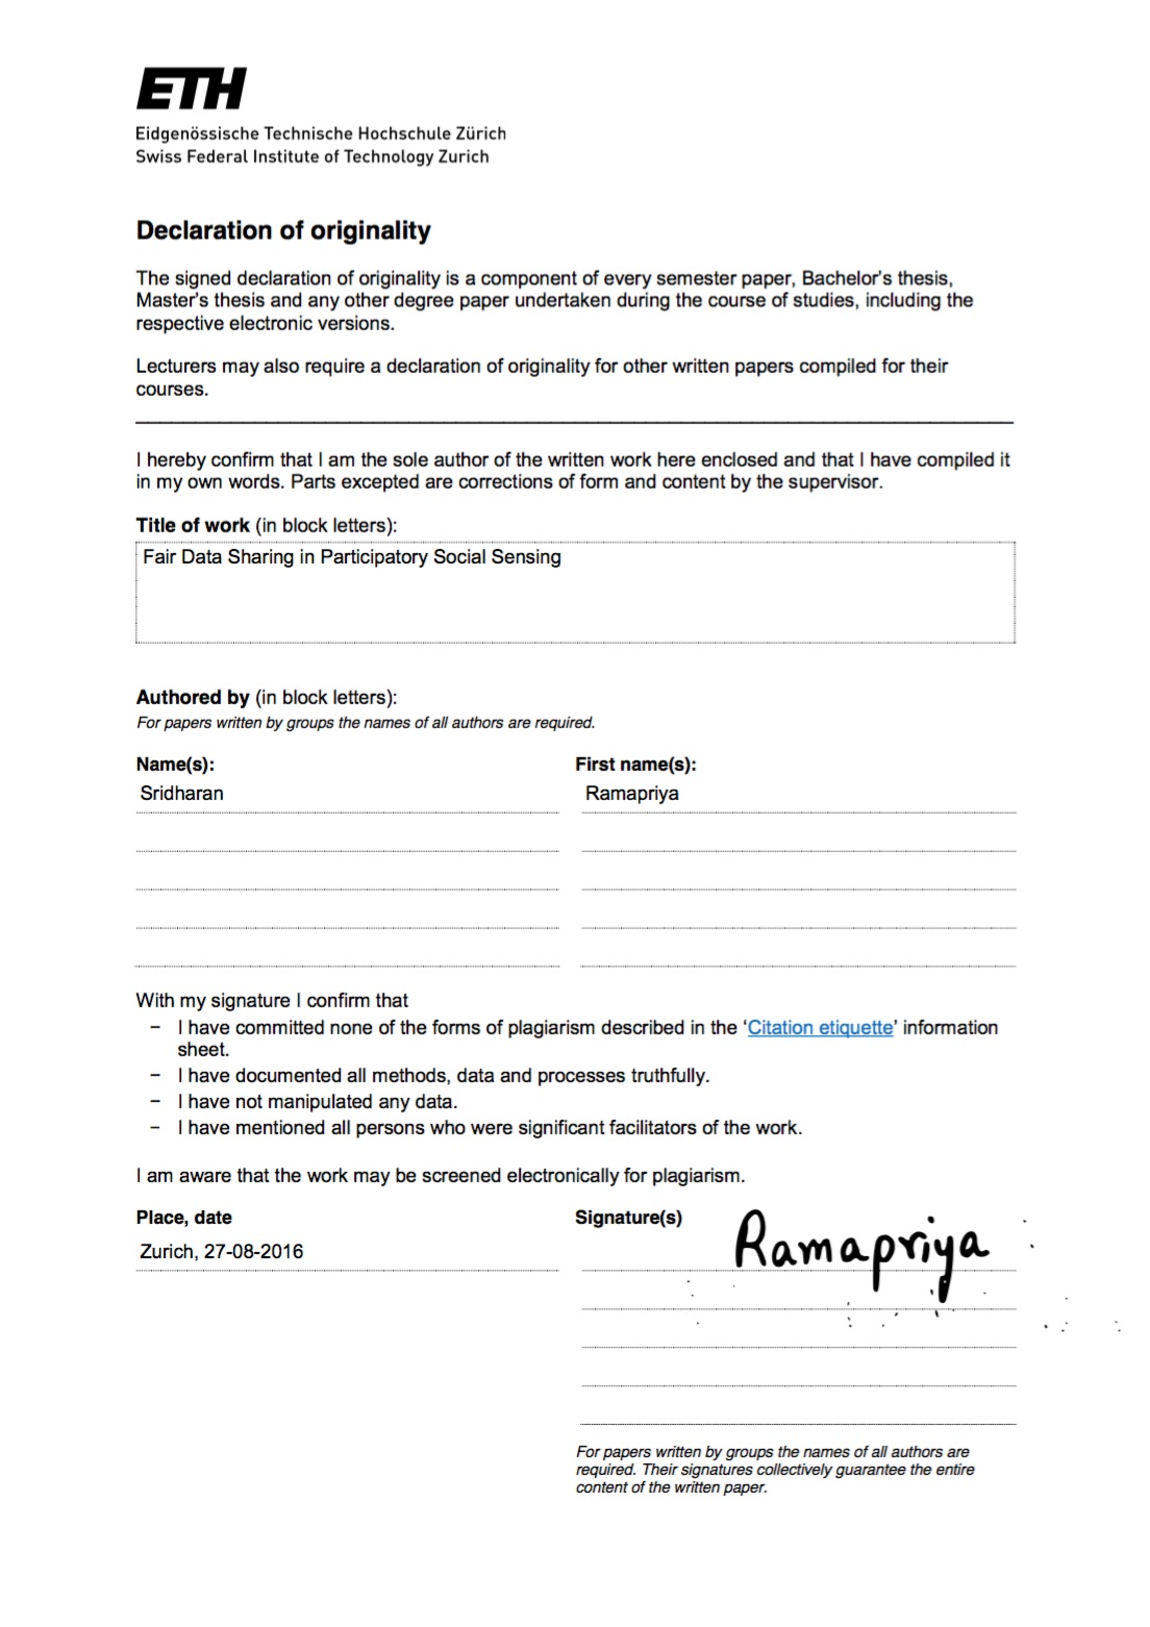
\includepdf[pages={-}]{declaration-originality.pdf}

\end{document}
